\documentclass[preview]{standalone}
\usepackage{tkz-graph}
\begin{document}

\begin{figure}[ht]
\center
 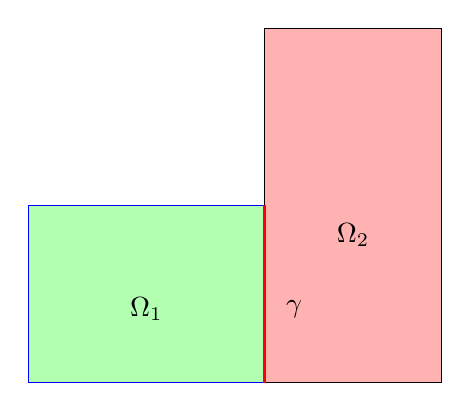
\begin{tikzpicture}[scale=0.75]

   \fill [green!30] (0,0) -- (0,3) -- (4,3) -- (4,0) -- (0,0);
   \draw [blue] (0,0) -- (0,3) -- (4,3) -- (4,0) -- (0,0);

   \fill [red!30] (4,0) -- (4,6) -- (7,6) -- (7,0) -- (4,0);
   \draw [black] (4,0) -- (4,6) -- (7,6) -- (7,0) -- (4,0);

   \draw [red, line width=1pt] (4,0) -- (4,3);

   \draw(2,1.25) node {$\Omega_1$}; 
   \draw(5.5,2.5) node {$\Omega_2$}; 
   \draw(4.5,1.25) node {$\gamma$}; 

 \end{tikzpicture}
\end{figure}





\end{document}



После: convert pdf to png
https://convertio.co/pdf-png/



 






